\section{Data Analysis}

The inelastic scattering of a WIMP with the nucleus of $^{129}$Xe produces an energy deposit via nuclear recoil with subsequent emission of  
a 39.6~KeV de-exitation photon. 
The largest fraction of the energy released in the event is via electronic recoil (ER) due to the emitted photon, this represents an
unusual signature for this kind of detector and brings the signal to overlay a phase space region with large backgrounds.
The choosen region of interest for this analysis surrounds the 39.6~KeV line in the cS1-cS2 plane which is further divided into
sub regions, as shown in figure~\ref{fig:SR}.

Events are asked, other than falling in the defined region of interest, to fullfill several selection criteria:
quality selection aimed to reduce noise impact toghether with energy and threshold selection on S2,
selection of single scatter events and fiducial volume definitions are reported in detail in \cite{dataAnalysis}, this analysis follows
the selection reported there for Run-II, only few modification have been designed specifically for this analysis and discussed below. 
In particular, selection on S2 width as a function of drift time has been optimized on a sample of events from 40~KeV of AmBe 
and set to a 95\% acceptance on those type of events.  

Xinelastic\_analysis\_S2width0
Inelastic\_Xs2single0

say something on data used: DM, calibration ecc..

brief explaination of the signature, selection cuts, few words about acceptances, image of signal region and control region.

\begin{figure}[h]
  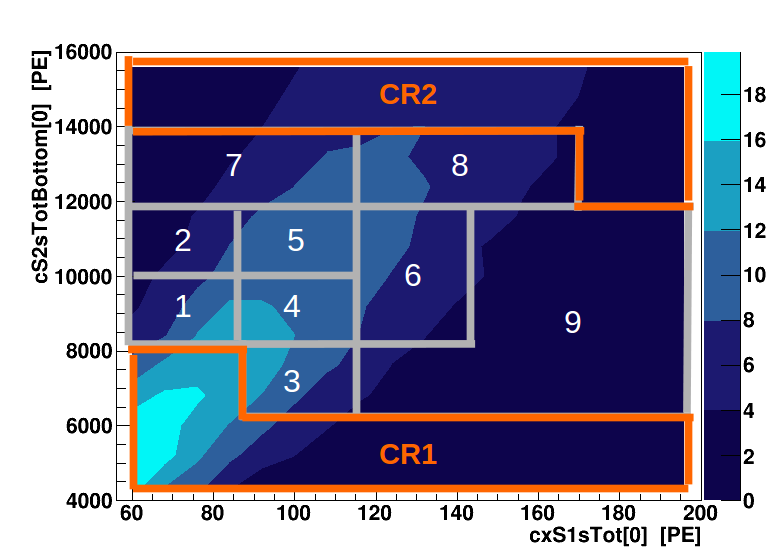
\includegraphics[width=\linewidth]{images/bkg_in_sr.png}
  \caption{Signal region and control region.}
  \label{fig:SR}
\end{figure}

\begin{figure}[h]
  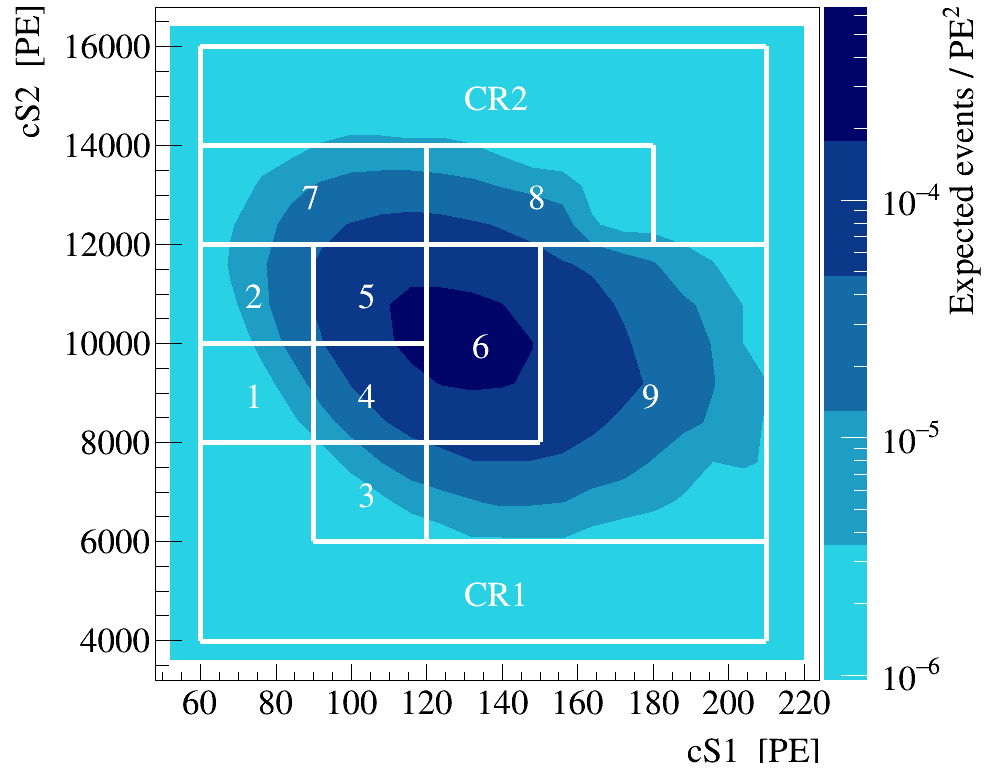
\includegraphics[width=\linewidth]{images/wimp_in_sr.png}
  \caption{Signal region and control region, for WIMP of mass 100~GeV.}
  \label{fig:SR2}
\end{figure}


\subsection{Signal Simulation} 

description of the simulated signal, few words about cross checks MC matching.


\subsection {Background Model}
Description of the data driven bkg model evaluation, few numbers on estimated background, words about cross checks with Th232.

%A citation in text uses the command \verb+\cite{#1}+ or
%\verb+\onlinecite{#1}+ and refers to an entry in the bibliography. 
%An entry in the bibliography is a reference to another document.
\subsection{Systematic Uncertainties}

few words, mainly a table summarizing uncertainties.

